%\documentclass[a4paper,12pt]{llncs}
%\usepackage[top=75pt, bottom=75pt, left=85pt, right=85pt]{geometry}

\documentclass{sig-alternate}
\usepackage{hyperref}
%\usepackage[stable]{footmisc}
\usepackage{epsfig}
\usepackage{textcomp}
\usepackage{times}


\usepackage{url}
\usepackage{listings}
\usepackage{comment}
\usepackage{subfigure}
\usepackage{amssymb}
\usepackage{amsmath}
\setcounter{tocdepth}{3}
\usepackage{graphicx}
\usepackage{soul,color}
\usepackage{url}
\usepackage{algorithm}


%\newcommand{\keywords}[1]{\par\addvspace\baselineskip
%\noindent\keywordname\enspace\ignorespaces#1}
\newcommand{\ie}{i.e.} 
\newcommand{\eg}{e.g.} 
\newcommand{\et}{et al. }

\begin{document}
\title{Short-term Water Demand Forecasting}

\numberofauthors{3}
\author{
\alignauthor
%Xiufeng Liu \\
%\affaddr{University of Waterloo}\\
%\email{xiufeng.liu@uwaterloo.ca}
%\alignauthor 
%Lukasz Golab \\
%\affaddr{University of Waterloo}\\
%\email{lgolab@uwaterloo.ca}
%\alignauthor 
%Ihab F. Ilyas \\
%\affaddr{University of Waterloo}\\
%\email{ilyas@uwaterloo.ca}
}
\maketitle

\begin{abstract}
\end{abstract}

\section{Introduction}

\section{Water Demand Forscasting Issues}

\subsection{Forcasting Models}

\subsection{Time Scales}

\subsection{Water Demand Patterns}

\section{Exploratory Analysis of Water Consumption Data}
\subsection{Weather in Abbotsford}
Abbotsford is a city located in the Lower Mainland region of British Columbia, Canada. Abbotsford is proximate to the Pacific Ocean, which provides milder winters, along with much greater rainfall than other regions at the same latitute. Abbotsford's winter and spring are cool, but relatively mild compared to most of Canada.   
The temperature starts to drop at the end of October. The rainy season starts at the end of October, and lasts lasts to April of the second year. November and December have the heaviest preciptation.  Summer in Abbotsford is relatively dry, and warm. The warmest month is August, which average daily high is $23.8 \,^{\circ}{\rm C}$, and sometimes as high as over $30 \,^{\circ}{\rm C}$. August averages only 20\% of November's rainfall, and only about 16\% of annual precipation falls. In Summer, it is common to receive little or no rainfall for weeks at a time.


\subsection{Water Use Distribution in Abbotsford}
The water consumption data is from  Abbotsford  city, British Columnbia, Canada from September 1, 2012 to August 31, 2013. Daily and hourly time-series data were collected from 25,294 customers,  distributed in six customer groups (see Figure~\ref{fig:avgwaterusagesummer}). There are 2013 215,172,496 data points in total for the hourly time-seriels data, and 9,232,310 data points for the daily time-series data (roughly 10GB in total). The residential customers are discriminated according to the house types, which are single family residential (SFRES) and multifamily residential (MFRES). As shown, the single family residential has the biggest share (79.61\%).

The climate data at the same period were downloaded from from Environment Canada (https://weather.gc.ca). The data contains the weather temperature at hourly resolution, and the rainfall at daily resolution.
\begin{figure*}[htp]
\centering
\begin{minipage}[b]{0.35\linewidth}
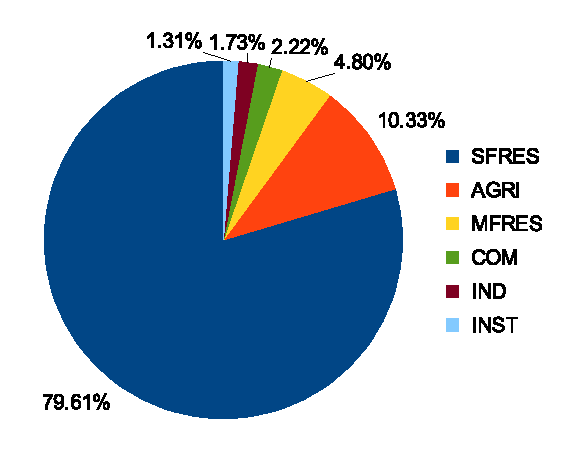
\includegraphics[width=0.9\textwidth]{images/watercustomergroups}
\vspace{-5pt}
\caption{Sizes of customer group}
\label{fig:watercustomergroups}
\end{minipage}
\begin{minipage}[b]{0.39\linewidth}
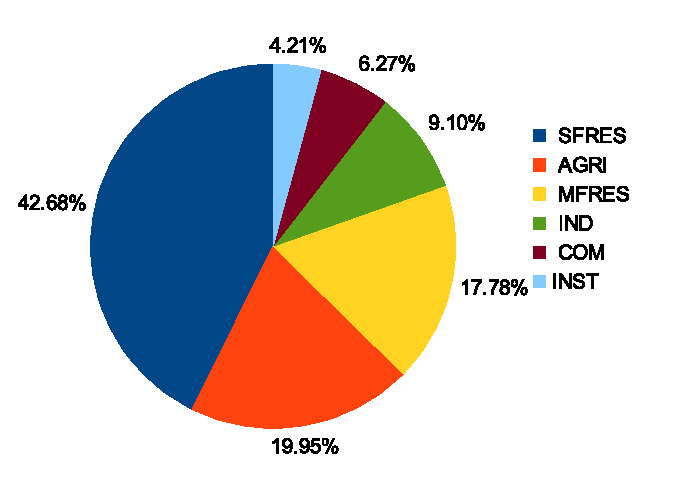
\includegraphics[width=0.9\textwidth]{images/waterconsumptiondist}
\vspace{-5pt}
\caption{Water consumption distribution}
\label{fig:waterconsumptiondist}
\end{minipage}
\end{figure*}




\begin{table*}[htp]
\centering
\caption{Sizes of customer types and the water consumption}
\begin{tabular}{p{2cm}p{2cm}p{2cm}p{2cm}p{2cm}p{2cm}}
\hline
                        & \multicolumn{2}{c}{Customer Types}                            &                      & \multicolumn{2}{c}{Water Consumption}                                    \\ \cline{2-3} \cline{5-6} 
                        & \multicolumn{1}{c}{Size} & \multicolumn{1}{c}{Percentage, \%} & \multicolumn{1}{c}{} & \multicolumn{1}{c}{Consumption, $m^3$} & \multicolumn{1}{c}{Percentage, \%} \\ \hline
\textbf{SFRES}          & 20,136                   & 79.61                              &                      & 5,158,189.4                         & 42.68                              \\
\textbf{AGRI}           & 2,612                    & 10.33                              &                      & 2,411,693.3                         & 19.95                              \\
\textbf{MFRES}          & 1,215                    & 4.80                               &                      & 2,148,880.4                         & 17.78                              \\
\textbf{COM}            & 561                      & 2.22                               &                      & 758,081.3                           & 6.27                               \\
\textbf{IND}            & 438                      & 1.73                               &                      & 1,099,533.5                         & 9.10                               \\
\textbf{INST}           & 332                      & 1.31                               &                      & 509,298.9                           & 4.21                               \\ \hline
\textit{\textbf{Total}} & 25,294                   & 100                                &                      & 12,085,676.9                        & 100                                \\ \hline
\end{tabular}
\label{tab:custgroupandconsump}
\end{table*}

\begin{figure*}[htp]
\centering
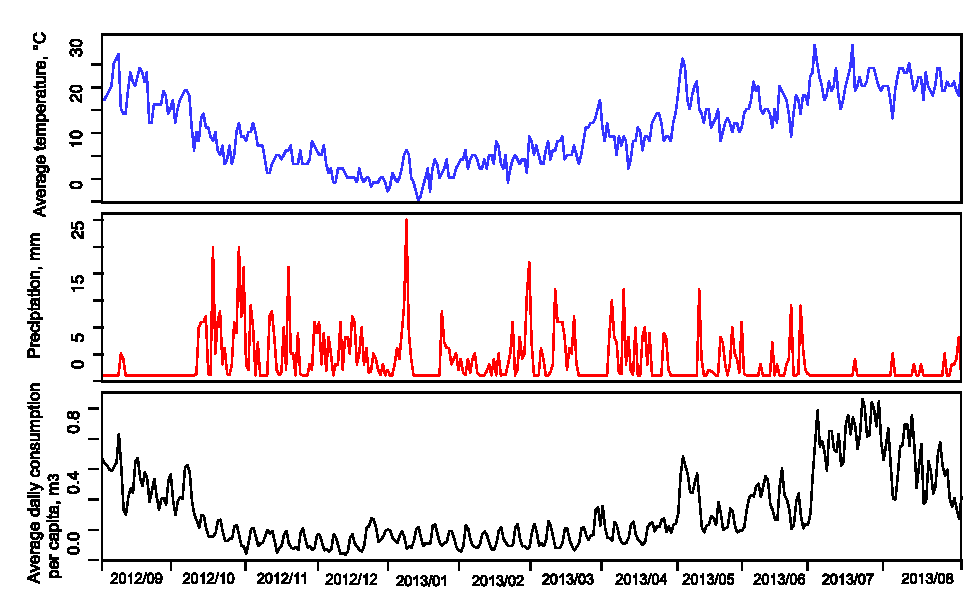
\includegraphics[width=0.8\textwidth]{images/weathervariableinwaterdemand}
\caption{The average daily profile of residential water consumption}
\label{fig:dailyprofile}
\end{figure*}




\subsection{Residential Water Use}
Approximately two-thirds of the water used in Abbotsford is for residential purposes, 42.68\% by the residents of single-family homes. In a spatially weighted regression analysis of single-family residential water demand at the census tract level, Wentz and Gober (2007) found that four variables--average household size, the percent of homes with a swimming pool, average lot size, and average percent of lots covered with mesic (turf) vegetation-explained more than 80\% of the spatial variation in metered water use. Larger household size increases indoor water use for such purposes as toilet flushing, showers, laundry, and dishwashing, although Arbu\'{e}s et al. (2003) note the tendency for less-than-proportional increases in use because of economies of
scale in water use. Swimming pools, lot size, and vegetation type account for outdoor use from pool evaporation and garden irrigation. We anticipate that residential water use is climate sensitive because of the
heavy reliance on outdoor uses in Abbotsford's water portfolio.

%In a study of the effect of the urban heat island on water use in Phoenix, Guhathakurta et al. (2005) examined the spatial effects of June nighttime temperature on residential water use, controlling for the presence of pools, vegetation type, size of house and lot, number of residents, and other socioeconomic, demographic, and housing variables. The effect of temperature was statistically significant, and the regression co-efficient indicated that an increase of 1°C resulted in an increase in household water use of 4.61 kL annually. In an environment in which the typical residence uses more than 600 kL of water, this constitutes 0.77\% of annual use for every 1°C of urban heating. With the heat-island effect exceeding 6°C, residential water use can be affected by over 4.5\%.


We show the daily time-series of the residential water usage in Figure~\ref{sfrestimeseries}. we could observer that the water usage shows periodicity in the days of a week. From Monday--Friday, the consumptions are lower than the weekend, and the holidays, propably for the reason that in the weekend and holiday people stays more time at home, thus use more water. In addition, we could observer that in summer time (May - October) the consumption are higher than winter time (November--April) which is probably due to the temperature effect. For example,  households grow the flowers in outdoors in summer, which need to water the flowers,  wash the care, or fill the swimming pools. Another climate effect we might consider is the effect of rainfall. For example, due to the rainfall, the water consumption might be reduced, \eg, people can save the water for watering the flowers in outdoor.




\begin{figure*}[htp]
\centering
\begin{minipage}[b]{0.4\linewidth}
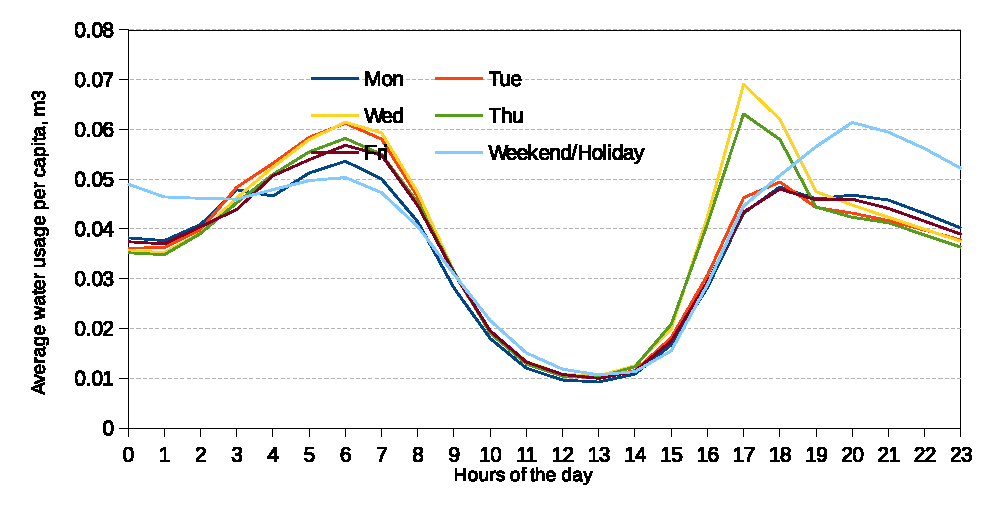
\includegraphics[width=1.0\textwidth]{images/avgwaterusagesummer}
\vspace{-15pt}
\caption{Daily pattern of hourly water demand in Summer}
\label{fig:avgwaterusagesummer}
\end{minipage}
\hspace{5pt}
\begin{minipage}[b]{0.4\linewidth}
\includegraphics[width=1.0\textwidth]{images/avgwaterusagewinter}
\vspace{-15pt}
\caption{Daily pattern of hourly water demand in Winter}
\label{fig:avgwaterusagewinter}
\end{minipage}
\end{figure*}

\begin{figure*}[htp]
\centering
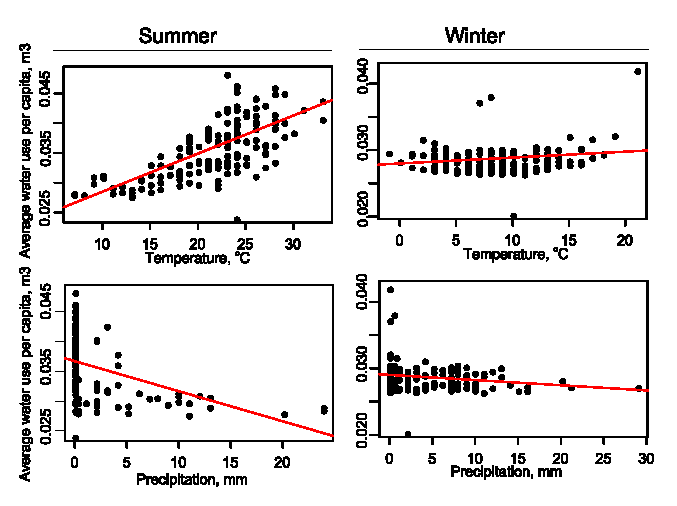
\includegraphics[width=0.8\textwidth]{images/waterusgexogvar}
\vspace{-5pt}
\caption{The effect of weather temperature and rainfall on water consumption}
\label{fig:waterusgexogvar}
\end{figure*}

\begin{figure*}[htp]
\centering
\begin{minipage}[b]{0.4\linewidth}
\includegraphics[width=1.0\textwidth]{images/hourlybaseloadsummer}
\vspace{-15pt}
\caption{Hourly baseload in Summer}
\label{fig:hourlybaseloadsummer}
\end{minipage}
\hspace{5pt}
\begin{minipage}[b]{0.4\linewidth}
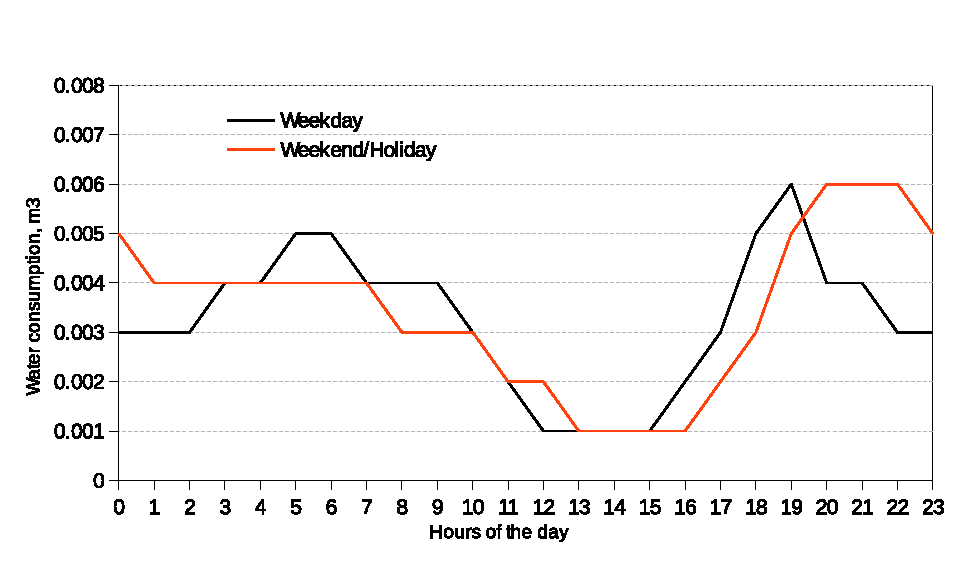
\includegraphics[width=1.0\textwidth]{images/hourlybaseloadwinter}
\vspace{-15pt}
\caption{Hourly baseload in Winter}
\label{fig:hourlybaseloadwinter}
\end{minipage}
\end{figure*}



\section{Model for Residential Water Demand Forecasting}
\subsection{Basis for Water Demand Forecasting}
For the residential water demand, many variables are considered influential and relevant in determining the water usgage. we refer to a report prepared for the Water Research Foundation by Coomes et al. (2010), in which the authors tested the effect of 26 variables on average daily water use for 293 residential customers of the Louisville Water Company.

The variables range from socio-economic to various derivatives of weather-related variables. Examples of these weather-related variables and how they are used can be found in Coomes et al. (2010) and Brekke et al. (2002).   The availability and choice of these independent variables can also influence the forecasting models used. For instance, whereas population projections and per capita demand are the drivers for unit rate models, these have no consideration when exponential smoothing or Box-Jenkins models are formulated

%Although “A good understanding of the factors influencing demand and reliable estimates of the parameters describing demand behavior and consumption patterns are prerequisites [to a good forecast]” (Burney et al. 2001), the enormity of these variables can create frustration for water utility mangers. As an illustration of the size and variability of the variables that can be considered,

We model the water consumption, $W_i$, into base load and seasonal load, which is as follows:
\begin{equation}
D_i = B_i + S_i 
\end{equation}

\subsection{Base Load}
The base load represents the weather insensitive portion of the total water use. The base load mainly are due to the use of daily use of living, such as drinking, toilet, bath and washing. The base use are unlikely to change abruptively, but might change slowly, \eg, placing more water efficient appliance such as new washing machine.  Therefore, the base use is assumed to be a fixed percentiled consumption of hourly flows in household for weekdays and weekends/holidays. We use 10 percentiled water usage as the base load, also adopted by \cite{zhou2002}. We derive the base load as follows: For the hourly base load, we aggregate the hourly readings of all residential customers at each hour of the day for each month, then calculate the lower ten percentile values. For the daily base load, we aggregate the daily readings of each workday of the week, and the weekend/holiday for all the households, then calcuate the ten percential value separately. The hourly base loads descriminated by Summer and Winter are shown in Figure~\ref{fig:hourlybaseloadsummer} and \ref{fig:hourlybaseloadwinter}. The daily base load for Summer and Winter are show in Figure~\ref{fig:dailybaseload}.
\begin{figure}[htp]
\centering
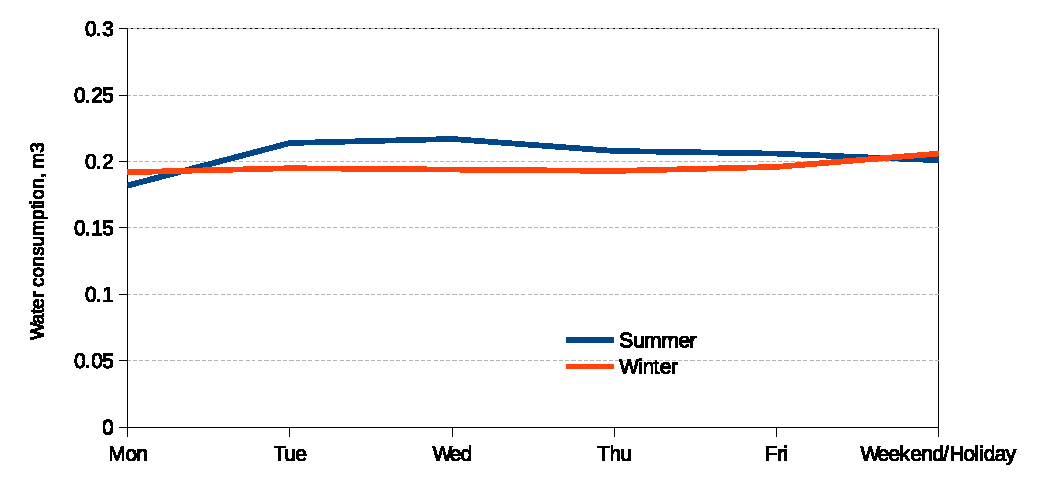
\includegraphics[width=0.45\textwidth]{images/dailybaseload}
\vspace{-5pt}
\caption{Daily baseload}
\label{fig:dailybaseload}
\end{figure}

\subsection{Daily Seasonal Load}
The daily seasonal load represents the weather sensitive portion of the total use of a day, \ie, the daily load subtracted by the base load, denoted as $S_i=D_i - B_i$. We use the periodic Auto-Regression with eXogenous variables (PARX) \cite{omid} to model the daily seasonal load. The period is weekly, and the seasons are the week days. Since the social and economic metric are avialble in our data, such as the price of water, and size of household, we therefore consider the climat impact on the residential water use. There are several environment variables including weather temperature, precipiutation and the number of days which precipitation exceede 0.2mm. We take these environmental factors as the exogenous vaiable in the PARX model. Thus, the model for daily seasonal load can be expressed as:
\begin{equation}
S_d = \sum_{i=1}^{p} \phi_{s,i} S_{d-i} + \beta_s h(T_d) + \psi_s g(R_d) + \eta_s f(t) + \epsilon_s,  \quad d \in s
\end{equation}
where $s$ is the season index;  $\phi_{s,i}, \beta_s, \psi_s \eta_s$  are the model parameters, and $\epsilon_s$ is the white noise;  $S_d$ represents the water consumption at a particular day $d$ in a week, and $d=0,...,6$ representing Sunday, Monday, ..., Saturday; $p$ is the order of auto-regression; $s$ is the season index; $h(T_t)$,  $g(R_t)$, and $f(nd)$ are the functions of weather temperature and rainfall effects. Most of the current studies model the weather variables to the water assumption linearly, such as \cite{zhou2002,schleich,bougadis}. However, Maidment and Miaou criticized the common linear approach, and suggest that the weateher vaiable, rainfall, has a dynamic effect, which reduces water demand initiallly, but the effect diminishes over time. Inspired by their suggestion, we set a thredhold value for each of the weather variables, which limit the effect of each weather variable. 
\[ h(T_d) = \left\{ 
  \begin{array}{l l}
    T_d - \tau & \quad T_d>\tau\\
    0 & \quad \text{Otherwise}
  \end{array} \right.\]
where $T_t$ is the maximum temperature at the week day $d$, and $\tau$ the thredhold of temperature effect. We adopt the 20 cesues degree as the thredhold value.
\[ g(R_t) = \left\{ 
  \begin{array}{l l}
    \gamma  & \quad R_t>\gamma\\
    R_t & \quad  \text{Otherwise}
  \end{array} \right.\]
where $R_t$ is the preciptation at the week day $t$, and $\gamma$ is the thredhold. 

\[
f(t) =  \left\{ 
  \begin{array}{l l}
    \zeta - t & \quad \zeta <t\\
     0 & \quad \text{Otherwise}
  \end{array} \right.\]  
where $t$ is the number of days since the the day with reprecition at least 0.2mm; and $\zeta$ is the thredhold value that we set to 3 days.

Akaike Information Criterion is used to choose the order of the autoregressive model. We use OLS to method  to fit the model.
\subsection{Hourly Seasonal Load}
-- No hourly rainfall data


\section{Results}
\subsection{The evaluation statistics}

\[
RSME = \frac{1}{n}\sqrt{\frac{1}{b} \sum_{i=1}^{n} e_i^2}
\]
\[
MAE = \frac{1}{n} \sum_{i=1}^{n}|\frac{e_i}{V_{obs}}|
\]

\subsection{Compare with the linear model}
We now use daily single family residential (SFRES), and weather data to compute the coefficients. We set the temperature thredhold value $\tau$ as 20 celsius degree, and the thredhold value of rainfall $\gamma$ as 1 mm preciptation.



\medskip
\begin{thebibliography}{1}

\bibitem{zhou2002}
Zhou, S. L., T. A. McMahon, A. Walton, and J. Lewis. "Forecasting operational demand for an urban water supply zone." Journal of Hydrology 259, no. 1 (2002): 189-202.

\bibitem{schleich}
Schleich, J., and Hillenbrand, T. (2009). Determinants of residential water demand in Germany. Ecological Economics, 68(6), 1756-1769.

\bibitem{bougadis}
Bougadis, John, Kaz Adamowski, and Roman Diduch. "Short‐term municipal water demand forecasting." Hydrological Processes 19.1 (2005): 137-148.

\bibitem{ibmbenchmark}
Ten Million Meters Scalable to One Hundred Million Meters for Five Billion Daily Meter Readings. Sept. 2011.

\bibitem{omid}
Ardakanian, O., Koochakzadeh, N., Singh, R. P., Golab, L., and Keshav, S. (2014). Computing Electricity Consumption Profiles from Household Smart Meter Data. In EDBT/ICDT Workshops (pp. 140-147).

\end{thebibliography}



\end{document}
